
\newcommand{\exampleFigure}[5]{
\begin{figure}[{#5}]
\begin{center}
\hspace*{-0.08\textwidth}
\includegraphics[clip, trim=0cm 0cm 0cm 0.85cm, width=1.1\textwidth]{chapters/3-Algorithms/examples/#1/#1#2.pdf}
\vspace{-25pt}
\caption{{#4}}
{#3}
\end{center}
\end{figure}
}

\newcommand{\exampleStepCommon}[4]{
\exampleFigure{#1}{#2}{#3}{#4}{h}
}

\newcommand{\makeCaption}[4]{Example: Algorithm variant \MaskVar{\uppercase{#1}} with $\maxerror={#2}$ and $\win={#3}$. Step {#4}.}

\newcommand{\commonIntro}[4]{Example: {#4}. Variant \MaskVar{\uppercase{#1}} with $\maxerror={#2}$. Step~{#3}.}
\newcommand{\makeCaptionIntroPWLH}[3]{\commonIntro{#1}{#2}{#3}{checking the valid hull condition}}
\newcommand{\makeCaptionIntroCA}[3]{\commonIntro{#1}{#2}{#3}{key steps of the coding algorithm}}
\newcommand{\makeCaptionIntroSF}[3]{\commonIntro{#1}{#2}{#3}{key steps of the coding algorithm}}


\newcommand{\exampleStepPCA}[4]{
\exampleStepCommon{#1}{#2}{#3}{\makeCaption{#1}{1}{4}{#4}}
}

\newcommand{\exampleStepGAMPS}[4]{
\exampleStepCommon{#1}{#2}{#3}{\makeCaption{#1}{0}{256}{#4}}
}

\newcommand{\exampleStep}[4]{
\exampleStepCommon{#1}{#2}{#3}{\makeCaption{#1}{1}{256}{#4}}
}

\newcommand{\exampleStepMany}[4]{
\exampleFigure{#1}{#2}{#3}{\makeCaption{#1}{1}{256}{#4}}{H}
}


%%%%%%%%%%%%%%%%%%%%%%%%%%%%%%%%%%%%%%%%%%%%%%%%%%%%%
%%%%%%%%%%%%%%%%%%%%%%%%%%%%%%%%%%%%%%%%%%%%%%%%%%%%%
%%%%%%%%%%%%%%%%%%%%%%%%%%%%%%%%%%%%%%%%%%%%%%%%%%%%%

\newcommand{\examplelinear}{
\centering
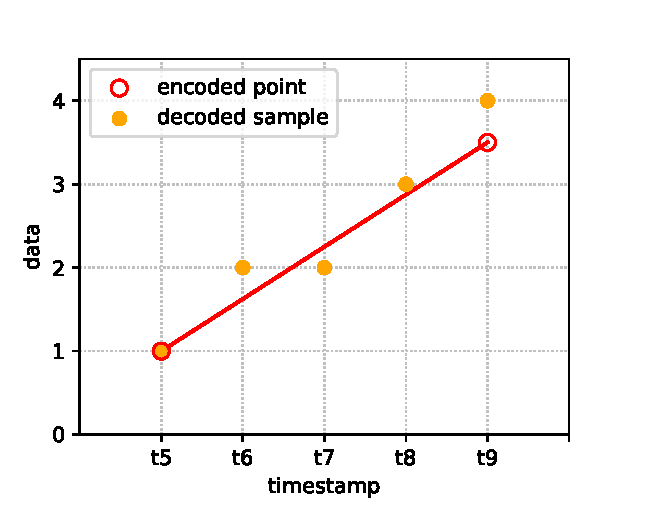
\includegraphics[width=1.2\textwidth]{chapters/3-Algorithms/examples/linear.pdf}
\vspace{-5pt}
\begin{minipage}{1.17\textwidth}
\captionof{figure}{Example of the auxiliary routine \decodeSegment\ for linear model algorithms.}
% \captionof{figure}{Example: auxiliary routine \decodeSegment\ for linear model algorithms.}
\label{example:linear}
\end{minipage}
}

\newcommand{\examplePWLH}{
\begin{figure}[h]
% \centering
\hspace{-30pt}
\begin{minipage}{.55\textwidth}
  \centering
  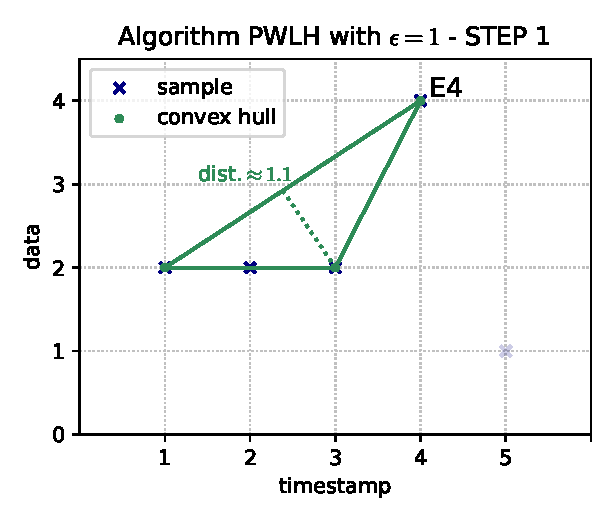
\includegraphics[clip, trim=0cm 0cm 0cm 0.9cm,width=1.0\linewidth]{chapters/3-Algorithms/examples/pwlh_intro/pwlh1.pdf}
  \vspace{-25pt}
  \captionof{figure}{\makeCaptionIntroPWLH{pwlh}{1}{1}}
  \label{example:pwlhIntro1}
\end{minipage}
\begin{minipage}{.55\textwidth}
  \centering
  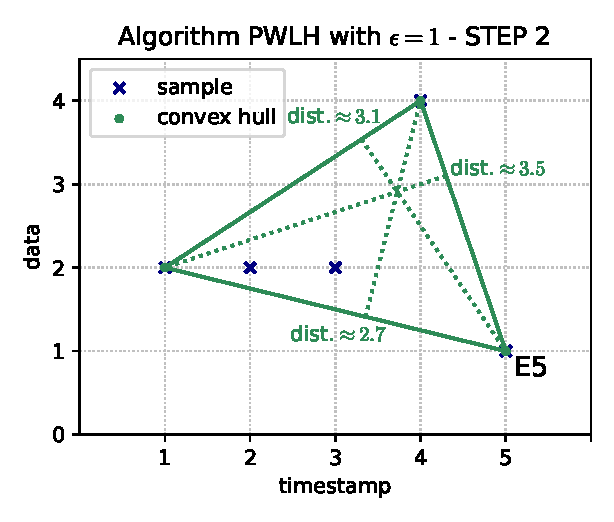
\includegraphics[clip, trim=0cm 0cm 0cm 0.9cm,width=1.0\linewidth]{chapters/3-Algorithms/examples/pwlh_intro/pwlh2.pdf}
  \vspace{-25pt}
  \captionof{figure}{\makeCaptionIntroPWLH{pwlh}{1}{2}}
  \label{example:pwlhIntro2}
\end{minipage}
\end{figure}
}

\newcommand{\exampleCA}{
\begin{figure}[h]
% \centering
\hspace{-30pt}
\begin{minipage}{.55\textwidth}
  \centering
  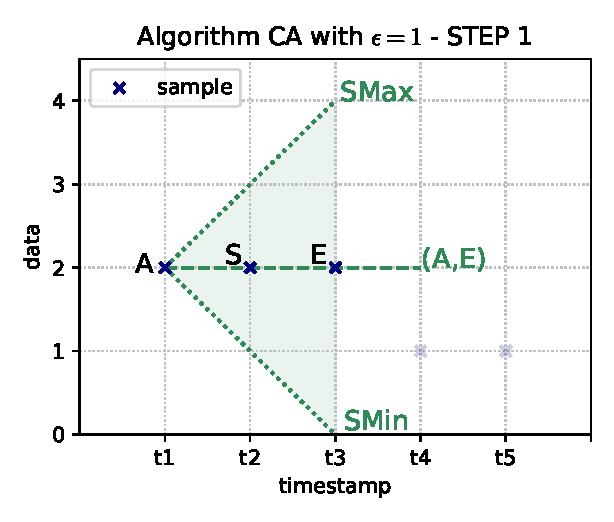
\includegraphics[clip, trim=0cm 0cm 0cm 0.9cm,width=1.0\linewidth]{chapters/3-Algorithms/examples/ca_intro/ca1.pdf}
  \vspace{-25pt}
  \captionof{figure}{\makeCaptionIntroCA{ca}{1}{1}}
  \label{example:caIntro1}
\end{minipage}%
\begin{minipage}{.55\textwidth}
  \centering
  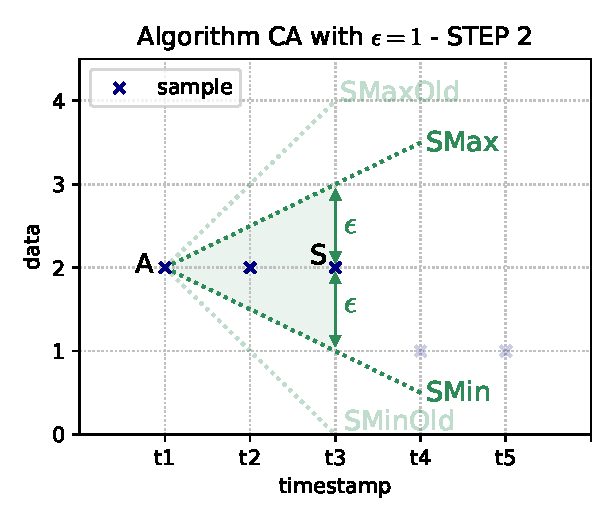
\includegraphics[clip, trim=0cm 0cm 0cm 0.9cm,width=1.0\linewidth]{chapters/3-Algorithms/examples/ca_intro/ca2.pdf}
  \vspace{-25pt}
  \captionof{figure}{\makeCaptionIntroCA{ca}{1}{2}}
  \label{example:caIntro2}
\end{minipage}
\end{figure}
}

\newcommand{\exampleSF}{
\begin{figure}[h]
% \centering
\hspace{-30pt}
\begin{minipage}{.55\textwidth}
  \centering
  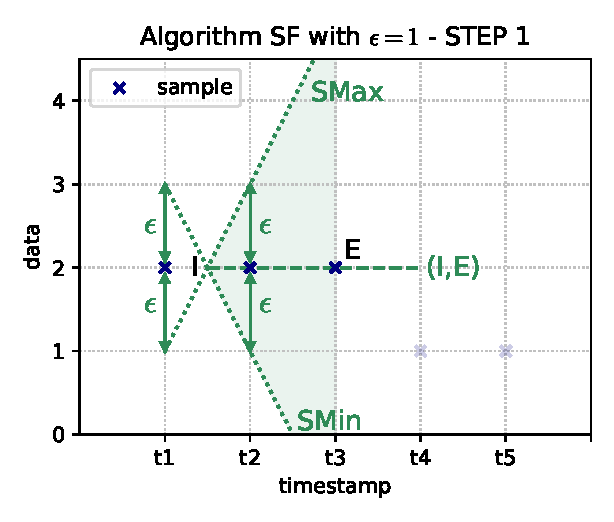
\includegraphics[clip, trim=0cm 0cm 0cm 0.9cm,width=1.0\linewidth]{chapters/3-Algorithms/examples/sf_intro/sf1.pdf}
  \vspace{-25pt}
  \captionof{figure}{\makeCaptionIntroSF{sf}{1}{1}}
  \label{example:sfIntro1}
\end{minipage}%
\begin{minipage}{.55\textwidth}
  \centering
  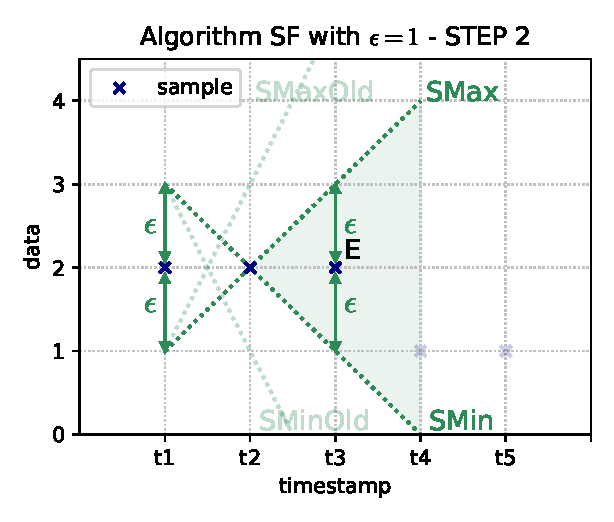
\includegraphics[clip, trim=0cm 0cm 0cm 0.9cm,width=1.0\linewidth]{chapters/3-Algorithms/examples/sf_intro/sf2.pdf}
  \vspace{-25pt}
  \captionof{figure}{\makeCaptionIntroSF{sf}{1}{2}}
  \label{example:sfIntro2}
\end{minipage}
\end{figure}
}
